%% Преамбула TeX-файла

% 1. Стиль и язык
\documentclass[utf8x, 12pt]{G7-32} % Стиль (по умолчанию будет 14pt)


% Остальные стандартные настройки убраны в preamble.inc.tex.
\sloppy

% Настройки стиля ГОСТ 7-32
% Для начала определяем, хотим мы или нет, чтобы рисунки и таблицы нумеровались в пределах раздела, или нам нужна сквозная нумерация.
%\EqInChapter % формулы будут нумероваться в пределах раздела
%\TableInChapter % таблицы будут нумероваться в пределах раздела
%\PicInChapter % рисунки будут нумероваться в пределах раздела

% Добавляем гипертекстовое оглавление в PDF
\usepackage[
bookmarks=true, colorlinks=true, unicode=true,
urlcolor=black,linkcolor=black, anchorcolor=black,
citecolor=black, menucolor=black, filecolor=black,
]{hyperref}

% Изменение начертания шрифта --- после чего выглядит таймсоподобно.
% apt-get install scalable-cyrfonts-tex

\IfFileExists{cyrtimes.sty}
    {
        \usepackage{cyrtimespatched}
    }
    {
        % А если Times нету, то будет CM...
    }

% TODO заметки
% https://tex.stackexchange.com/questions/9796/how-to-add-todo-notes
% \usepackage[colorinlistoftodos,prependcaption,textsize=tiny,obeyFinal]{todonotes}
\usepackage{xargs}
\newcommandx{\unsure}[2][1=]{\todo[linecolor=red,backgroundcolor=red!25,bordercolor=red,#1]{#2}}
\newcommandx{\change}[2][1=]{\todo[linecolor=blue,backgroundcolor=blue!25,bordercolor=blue,#1]{#2}}
\newcommandx{\info}[2][1=]{\todo[linecolor=OliveGreen,backgroundcolor=OliveGreen!25,bordercolor=OliveGreen,#1]{#2}}
\newcommandx{\improvement}[2][1=]{\todo[linecolor=Plum,backgroundcolor=Plum!25,bordercolor=Plum,#1]{#2}}
\newcommandx{\thiswillnotshow}[2][1=]{\todo[disable,#1]{#2}}

\usepackage{comment}

\usepackage{xcolor}
\usepackage{ifdraft}
\ifoptionfinal{
\newcommand{\hl}[1]{#1}
}{
\newcommand{\hl}[1]{\colorbox{yellow}{#1}}
}

\usepackage{graphicx}   % Пакет для включения рисунков
\graphicspath{ {charts/} }
\DeclareGraphicsExtensions{.jpg,.pdf,.png}
% С такими оно полями оно работает по-умолчанию:
% \RequirePackage[left=20mm,right=10mm,top=20mm,bottom=20mm,headsep=0pt]{geometry}
% Если вас тошнит от поля в 10мм --- увеличивайте до 20-ти, ну и про переплёт не забывайте:
\geometry{right=20mm}
\geometry{left=30mm}


% Произвольная нумерация списков.
\usepackage{enumerate}

\usepackage{float}
\restylefloat{table}

\setcounter{tocdepth}{2} %Подробность оглавления
%4 это chapter, section, subsection, subsubsection и paragraph
%3 это chapter, section, subsection и subsubsection
%2 это chapter, section, и subsection
%1 это chapter и section
%0 это chapter.

\usepackage{mathtext}
\usepackage[russian]{babel}



\begin{document}

\frontmatter % выключает нумерацию ВСЕГО; здесь начинаются ненумерованные главы: реферат, введение, глоссарий, сокращения и прочее.
\setcounter{page}{1}
\begin{center} 

\large Московский государственный университет имени М.В. Ломоносова\\
Факультет вычислительной математики и кибернетики\\
Кафедра интеллектуальных информационных технологий\\[5.5cm] 

\huge Методы анализа поведения пользователя в задаче обнаружения внутренних вторжений с помощью нейросетей \\[0.6cm] % название работы, затем отступ 0,6см
% \large Моделирование пользовательского поведения с помощью нейронных сетей для решения задачи обнаружения инсайдеров\\[3.7cm]


\end{center} 

\begin{flushright}
Александров В. В. \\
Царёв Д. В. \\
\end{flushright}


\vfill 

\begin{center} 
\large Москва 2020
\end{center} 

\thispagestyle{empty}

\thispagestyle{empty}

\mainmatter

\tableofcontents
\clearpage


% \chapter{Аннотация}

% Целью данной работы является изучение средств для создания системы автоматического обнаружения инсайдерских угроз по поведенческой информации пользователей.\\
% Рассмотрен ряд различных существующих решений, которые основаны на синтетическом наборе данных инсайдерских угроз CMU CERT. На основе анализа моделей, для разработки выбрана архитектура нейросетевой модели с LSTM-кодировщиком поведения и CNN-классификатора. Результаты нейросетевых моделей сравниваются с классическими алгоритмами машинного обучения.\\
% В процессе работы были испробованы различные техники и изменения для улучшения качества предсказаний моделей такие как применение embedding-слоя в LSTM-кодировщике, взвешенная функция потерь, использование Batch Normalization, добавление дополнительных признаков, в том числе признаков о содержимом файлов.

\chapter{Введение}

\textbf{Внутренние (инсайдерские) вторжения} — это вредоносные для организации угрозы, которые исходят от людей внутри организации, таких как работники, бывшие работники, подрядчики или деловые партнеры, имеющих доступ к информации о методах безопасности внутри организации, данных и компьютерных системах.\\

Инсайдерские угрозы в данный момент является серьезной проблемой для многих организаций. Их обнаружение является очень трудной задачей в силу того, что инсайдеры для злонамеренных действий используют доверенный им доступ, из-за чего они могут легко обходить системы внешней защиты информации.\\

Существует ряд технологий, для решения проблем инсайдерских угроз:\\
\begin{itemize}
\item DLP (Data Loss Prevention) – предотвращение утечек с помощью анализа потоков данных, пересекающих периметр информационной системы\\
\item SIEM (Security Information and Event Management) – анализ в реальном времени событий безопасности\\
\item IAM (Identity and Access Management) – управление учетными данными пользователей, системами контроля и управления доступом\\
\item UEBA (User and Entity Behavior Analytics) – анализ действий пользователя и принятие решения на основе исторических данных\\
\end{itemize}

DLP, SIEM и IAM системы способны бороться с инсайдерами только на самом последнем этапе утечки данных, когда инсайдер пытается провести эксфильтрацию данных. При этом, до этого момента инсайдер проходит стадии подготовки утечки, которая может длиться месяцами и в течение этого этапа инсайдер проявляет аномальное поведение. Поэтому существует отдельный класс решений UEBA, который направлен на анализ поведения пользователей и способны обнаруживать ранние признаки утечки информации.\\

Под поведенческой информацией понимается совокупность данных, которые описывают:\\
\begin{itemize}
\item Контекст – структурированные данные, описывающие атрибуты операций, которые пользователь выполняет с документами;
\item Контент – неструктурированные данные в виде содержимого документов, ассоциированные с операциями пользователя.
\end{itemize}

\section*{Актуальность задачи}

По отчетам Ponemon за 2020 год \cite{PonemonReport20182018} стоимость ущерба от инсайдерских угроз составляет 11,45 миллионов долларов в среднем за атаку. При этом средняя стоимость атак выросла на 31\% в два раза с 2018 года. По тому же отчету, частота инсайдерских инцидентов также заметно выросла. Также приводится, что из всех методов борьбы с инсайдерской угрозой UEBA системы лидируют по степени сокращения финансового ущерба. В среднем они сокращают 3,42 миллиона долларов. Это как раз связано с тем, что UEBA системы способны обнаруживать аномальное поведение пользователя на ранних этапах утечки информации. Это подтверждается в \cite{2019InsiderThreat}, где подчеркивается, что в силу того, что инсайдеры имеют мало препятствий, время с первых несанкционированных действий до обнаружения часто занимает месяцы и годы.\\ \\

Согласно McKinsey \cite{InsiderThreatHuman} из всех опубликованных в VERIS Community Database публичных случаях утечки информации за период с 2012 по 2017 год, в 50\% присутствовал элемент инсайдерской угрозы. При этом, 38\% случаев из этих наличествует злонамеренные действия инсайдеров. В отчете Verizon за 2019 год \cite{2019InsiderThreat} приводится, что 57\% взломов базы данных организации включают в себя инсайдерские угрозы.\\

Отчеты Haystax \cite{veriatoInsiderThreatReport}\cite{companyInsiderThreatReport} и Gartner \cite{EmergingInsiderThreat2018} подтверждают растущие опасения организаций по этому поводу и тренд на рост частоты атак инсайдеров.

Согласно отчету Gartner \cite{GartnerReportMarket2019} рынок самостоятельных UEBA-систем умирает, но в данный момент очень востребованы SIEM-системы, которые включают в себя UEBA.\\

По приведенным выше отчетам становится очевидной актуальность изучения и разработки моделей машинного обучения, способные определять ранние признаки аномального поведения корпоративных пользователей.

Существующие UEBA-решения нацелены в первую очередь на анализ структурированной контекстной информации о поведении пользователя которые включают в себя обычно данные об операциях с файлами, электронной почты, подключении новых устройств и данные из системного журнала ОС. Это объясняется тем, что анализ контентной информации намного более затруднителен из-за своей неструктурированности и очень большого объёма. В то же время, анализ контента позволяет выявлять случаи, при которых поведения пользователя остаётся таким же, но меняется содержимое файлов, с которыми он работает. Анализ только структурированной информации такие случаи выявить не может, что позволяет утверждать о ценности контента для рассматриваемой задачи. Актуальность анализа текстовых данных также подвтерждается отчётом Gartner \cite{GartnerReportMarket2019}.\\


\chapter{Постановка задачи}

\begin{enumerate}
	\item Реализация системы сбора поведенческой информации пользователя. Типы поведенческой информации:
	\begin{enumerate}
		\item контекст пользовательских операций;
		\item контент файлов;
	\end{enumerate}
	\item Исследование и разработка методов обнаружения аномального поведения пользователей на основе собираемой поведенческой информации.
\end{enumerate}

\chapter{Обзор существующих решений рассматриваемой задачи или ее модификаций}

Рассмотрим существующие методы построения моделей машинного обучения для задачи автоматического обнаружения инсайдерских угроз на основе поведенческих данных. Также рассмотрим доступные публичные наборы данных, которые потенциально могут быть использованы для обучения моделей.

\section{Обзор моделей}

Синтетический набор данных разработанный подразделением CERT Carnegie Melon University пользуется очень большой популярностью в исследованиях на данную тему. Поэтому, по умолчанию, во всех приведенных статьях ниже используется набор данных CERT версии 4.2. Также по умолчанию содержимое писем, файлов и вебсайтов из данного набора данных не используется.\\

В работе \cite{rashidNewTakeDetecting2016} используется скрытая марковская модель (Hidden Markov Model - \textbf{HMM}). Скрытая марковская модель представляет собой обычную марковскую модель, в которой модель выводит некоторый символ каждый раз перед переходом в следующее состояние. Модель называется скрытой, поскольку мы наблюдаем только выходы модели, а последовательность переходов состояний скрыта от нас.\\
В данной работе все действия пользователей кодируются числами. Затем действия собираются отдельно для каждого пользователя и сортируются по времени. На первых пяти неделях модель обучается (используется предположение, что за это время инсайдерского поведения не было), для последующих недель модель предсказывает вероятность аномальности поведения и только потом обучается. Поведение за неделю считается аномальным, если оно превышает заданный порог.\\
Эксперименты на CERT 4.2 после подбора гиперпараметров показали AUC ROC $0.83$.\\

В \cite{aldairiTrustAwareUnsupervised2019} также применяется метод обучения без учителя и задача обнаружения инсайдерских угроз ставится как задача обнаружения аномалий. В этой работе сравниваются два классических метода нахождения аномалий:\\
\begin{enumerate}
\item Isolation Forest (Изолирующий лес) - разновидность алгоритма случайного леса, в котором строятся случайные бинарные решающие деревья. Аномальными объектами считаются те, которые часто оказываются в листьях с низкой глубиной
\item Метод опорных векторов для одного класса (One Class SVM) представляет собой обычный SVM, в котором все данные имеют положительную метку. При оптимизации модель пытается вместить как можно больше объектов в как можно меньшую гиперплоскость. В результате получается граница, по одну сторону которой максимально плотно упакованы наблюдения из тренировочной выборке, а по другую будут находиться аномальные значения.\\
\end{enumerate}
Работа проводилась на наборе данных CERT. Моделям на вход подавались данные агрегированные по разным временным периодам - дням, месяцам, полугодиям и годам. Также в качестве дополнительного признака используется trust score (показатель доверия), который означает оценку аномальности пользователя для предыдущего периода. Авторы показывают, что этот признак заметно улучшает точность предсказаний моделей, особенно в случаях моделей, в которых данные агрегируются по малым периодам.\\

В статье \cite{luInsiderThreatDetection2019} применяется рекуррентная нейронная сеть LSTM для поиска аномалий в поведении пользователей.\\
%%% Описание LSTM %%%
\textbf{Long Short Term Memory (LSTM)} - разновидность рекуррентных нейронных сетей. Обучение рекуррентных сетей является трудной задачей из-за проблемы взрывающихся и затухающих градиентов. Более того, RNN не могут удерживать в ``памяти'' долговременные зависимости. Чтобы решить эту проблему были предложены LSTM сети, которые способны удерживать информацию в течение длительного времени. LSTM имеет три фильтра, которые помогают защищать и контролировать состояние ячейки. Фильтр входа (input gate) решает, какие значения следует обновить при подаче новой информации. Фильтр ``забывания'' (forget gate) определяет какую часть значений следует ``забыть'' и фильтр выхода (output gate) определяет какую часть значения можно вывести в качество выхода.\\
Шаг обновления LSTM:\\
\begin{align}
i_t = &\: \sigma(\mathbf{W_i}e_t+\mathbf{U_i}h_{t-1}+b_i)\\
f_t = &\: \sigma(\mathbf{W_f}e_t+\mathbf{U_f}h_{t-1}+b_f)\\
o_t = &\: \sigma(\mathbf{W_o}e_t+\mathbf{U_o}h_{t-1}+b_o)\\
g_t = &\: \tanh(\mathbf{W_g}e_t+\mathbf{U_g}h_{t-1}+b_g)\\
c_t = &\: f_t\odot c{t-1}+i_t\odot g_t\\
h_t = &\: o_t \odot \tanh(c_t)
\end{align}
где $\mathbf{W}$, $\mathbf{U}$ - обучаемые матрицы параметров, $e_t$ - входной вектор, $h_t$ - выходной вектор, $c_t$ - вектор состояния сети, $f_t$, $i_t$, $o_t$ - векторы вентилей.\\
В работе \cite{luInsiderThreatDetection2019} Каждый отдельный тип действия пользователей кодируется определенным числом. Последовательность закодированных действий разбивается на пересекающиеся блоки размера $n$ с помощью скользящего окна. Размер блоков является гиперпараметром. Далее последовательность блоков действий подается н вход LSTM-сети, которая пытается предсказать следующее действие пользователя. Предполагается, что при нормальном поведении пользователя, правильное действие пользователя попадает в $g$ наиболее вероятных предсказаний. $g$ также является гиперпараметром.\\
В работе проведены эксперименты, которые показывают, что LSTM действительно обучается паттернам поведения пользователей и находить аномальное поведение. Наилучший результат при подборе гиперпараметров: точность - $0.84$ и полнота - $0.60$.\\
В статье приводится предположение, что некоторые случаи, в которых модель ошибочно не распознала аномальное поведение, можно разрешить с помощью анализа контента.

В \cite{noeverClassifierSuitesInsider2019} было испробовано множество различных семейств алгоритмов машинного обучения. В этой статье приводится к заключению, что алгоритмы случайного леса и бустинга показывают наилучшие результаты. Важно отметить, что они в качестве признаков также использовали сентимент-анализ текста электронной почты и содержания посещенных сайтов.

При применении моделей машинного обучения качество моделей очень сильно зависит от признаков, которые были вручную сгенерированы исследователями. Однако в последнее время наблюдается очень большой интерес к нейронным сетям, в том числе из-за того, что они способны автоматически выучивать хорошее признаковое представление данных. Поэтому и в данной теме множество последних работ использует нейросети.\\

В работе \cite{brdiczkaProactiveInsiderThreat2012b} используется информация о социальном графе для нахождения аномалий в нем и поведенческая информация пользователей для психологического профилирования. Интересно отметить, что в данной работе в качестве данных использовались данные из популярной онлайн многопользовательской игры World of Warcraft(WoW). Они собрали данные о социальном графе игроков внутри игры и его изменениях за шесть месяцев. Авторы с помощью своего методы пытались предсказать то, что игрок в скором времени покинет гильдию (социальную группу внутри игры). В пользу необычного выбора набора данных приводится, что данных много, содержат в себе зловредные поведения, публичны и не ограничены правилами конфиденциальности. Авторы утверждают, что предложенный ими метод можно применять также и на реальных предприятиях.\\

В статье \cite{yuanInsiderThreatDetection2018b} используется следующий подход: сначала LSTM выучивает поведение пользователя по его действиям и извлекает временные признаки, затем извлеченные признаки подаются на вход CNN классификатору.\\

%%% Описание CNN %%%
\textbf{Сверточные нейронные сети CNN} - специальная разновидность архитектур нейронных сетей, в которой слои, выполняющие свертку, чередуются со слоями субдискретизации. На данный момент, CNN является одним из лучших алгоритмов по распознаванию и классификации изображений.\\

Поведения пользователя рассматривается как последовательность действий и действия одного пользователя соответствует одному "предложению", как в обычных NLP задачах. Все действия пользователя перед подачей на вход модели one-hot кодируются. После подачи каждого действия каждый скрытый слой LSTM выдает вектор, который выражает текущее состояние сети в пространстве малой размерности. Выходы последнего слоя собираются в одну матрицу, которая затем приводится к фиксированному размеру с помощью отбрасывания лишних векторов в случае длинных последовательностей действий и заполнения нулями в случае коротких последовательностей. Полученная матрица подается на вход CNN сети, которая в свою очередь предсказывает аномальность поведения. Авторы пишут, что их метод показал $AUC ROC=0.9449$ на отложенной выборке CERT.\\

В другой работе \cite{saaudiInsiderThreatsDetection2019} используется обратный подход. В ней CNN с одномерными сверточными слоями сначала пытается извлечь признаки, затем они подаются на вход LSTM для классификации. Значимое отличие от предыдущей работы заключается в том, что отображение поведения пользователей происходит с помощью представления каждого отдельного действия вектором малой размерностью. Значения этого вектора характеризуются соседними действиями, которые обычно встречаются вместе с ним. Авторы не указывают точно какой метод они использовали, но по описанию это очень похоже на популярный подход word2vec \cite{mikolovEfficientEstimationWord2013a}. Также авторы использовали технику SMOTE \cite{chawlaSMOTESyntheticMinority2002} для семплирования объектов малого класса и исправления сильного дисбаланса классов в наборе данных. SMOTE генерирует синтетические данные, которые похожи на $k$ ближайших соседей малого класса.\\

Обе работы \cite{saaudiInsiderThreatsDetection2019} и \cite{yuanInsiderThreatDetection2018b} ставят свою задачу как бинарную классификацию, в которой алгоритму необходимо определить аномальность поведения пользователя за некоторый промежуток времени (в обеих статьях рассматривают данные по дням)

В работе \cite{yuanAttentionBasedLSTMInsider2019} исследуется применение механизма \textbf{Attention} (внимание) для задачи обнаружения инсайдеров. Этот механизм позволяет сети обращать особое внимание для некоторых важных действий. Attention-слой в данной сети собирают выходы LSTM-слоя в один вектор, присваивая различный вес каждому выходу в зависимости от его важности. Вычисления в Attention-слоя следующие: \\
\begin{align}
\mathbf{u_t} = &\: \tanh (\mathbf{W_a}\mathbf{h_t}+\mathbf{b_a})\\
\alpha_t = &\: \frac{\exp (\mathbf{u_t^T}\mathbf{u_a})}{\sum_i \exp (\mathbf{u_i^T}\mathbf{u_a}}\\
\mathbf{v} = &\: \sum_t \alpha_t\mathbf{h_t}
\end{align}
где $\mathbf{W_a}$ - обучаемая матрица параметров, $\mathbf{u_a}$ - обучаемый вектор контекста, $\mathbf{h_t}$ t-ый выход из LSTM-слоя.\\
Полученный вектор $v$ подается на вход Softmax классификатору:
\begin{equation}
p(\hat{y}=k | \mathbf{v}) = \frac{\exp(\mathbf{W_k^T}\mathbf{v} + \mathbf{b_k})}{\sum^K_{i=1} \exp(\mathbf{W_i^T}\mathbf{v} + \mathbf{b_i})}
\end{equation}
где, $\hat{y}$ - предсказанный класс, $K$ - количество классов, $\mathbf{W_k}$ и $\mathbf{b_k}$ - обучаемые параметры для k-ого класса.\\
Как показали эксперименты в \cite{yuanAttentionBasedLSTMInsider2019}, добавление Attention увеличивает AUC ROC для LSTM и RNN сетей при использовании набора данных CERT.\\

Для поиска аномалий также возможно применение нейронных сетей из области распознавания изображений. Вдохновленные недавними успехами в применении нейросетей для анализа изображений для классификации вредоносных программ, \cite{gImageBasedFeatureRepresentation2019} применили этот подход для задачи обнаружении инсайдерской угрозы. В этой работе из набора данных CERT было вручную отобрано 20 признаков, и для каждого пользователя отдельно по этим признаком составлялись изображения 32 на 32 пикселей, которые подавались предобученной на ImageNet популярным нейросетевым моделям VGG16 и MobileNet. В результате было получено 99.32 точность и полнота на отложенной выборке.\\

В \cite{leggAutomatedInsiderThreat2017} строится трехуровневая система для обнаружения инсайдерских угроз. Первый уровень предполагает собой профилирование поведения пользователей и целых ролей в совокупности. На этом уровне срабатывает тревога при нарушении заданных правил.\\
 На следующем уровне для каждого пользователя собирается матрица дневных наблюдений, размерность которой уменьшается с помощью PCA. Последняя строка матрицы означает поведение пользователя в текущий день. В качестве оценки аномальности берётся расстояние последней строки до начала координат в новом пространстве. Вычисляется сразу множество оценок аномальности, каждая из которых соответствует собственному подмножеству используемых признаков и различному набору весов признаков. Тревога на этом уровне срабатывает, если какая-либо из оценок аномальности превышает заданные пороги.\\
 На третьем уровне анализируются полученные оценки аномальности, чтобы понять, насколько эти оценки необычны в сравнении с обычным поведением и, при необходимости, дать тревогу. Авторы предлагают для этого сразу множество вариантов.\\
Следует отметить, что в данной работе также учитывается контент файлов, но лишь как дополнительный компонент системы. Авторы предлагают использовать классический метод ``мешок слов'' или технику Linguistic Inquiry and Word Count (\textbf{LIWC}) \cite{tausczikPsychologicalMeaningWords2010}, которая заключается в распределение слов по категориям, имеющие смысл с точки зрения психологии.\\
В работе для обучения CERT, без указания точной версии, а для валидации использовался их собственный синтетический набор данных, похожий по структуре на CERT.
\\

% Несмотря на то, что набор данных CERT кроме информации о совершенных действиях пользователя также содержит сгенерированный контент файлов, писем и веб-сайтов, в подавляющем большинстве работ контент файлов не анализируется или используется лишь как дополнительный модуль, как например в \cite{leggAutomatedInsiderThreat2017}, где контент анализировался с помощью техники "мешок слов". Это обусловлено тем, что в наборе данных CERT до пятой версии генерации происходила с помощью ``мешка слов'' по смеси тем пользователя. То есть контент представляет собой неупорядоченный набор ключевых слов, которые которые представляют темы, интересующие пользователя. Поэтому использовать техники, учитывающие порядок слов, как например N-граммы, не имеет смысла.\\

% Однако последние работы в сфере NLP сделали большой прогресс в получении ``осмысленного'' признакового представления текстовых данных основанные на семантическом значении слов. Техники word2Vec\cite{mikolovEfficientEstimationWord2013a}, GloVe и ELMO позволяющие получать признаковое описание слов в пространстве малой размерности, позволили улучшить качество моделей для большинства NLP задач. Также в конце 2018 года появилась модель BERT \cite{devlinBERTPretrainingDeep2019}, которая улучшила качество работы по 6 различным NLP задачам. Обученный BERT также способен выдавать признаковое представление отдельных слов. Также в \cite{noeverClassifierSuitesInsider2019} отмечалось, сентимент-анализ содержимого писем и вебсайтов оказывает значительное влияние на качество моделей.\\

Также, как показано в статье \cite{yuanAttentionBasedLSTMInsider2019}, техника attention в применении к поведенческой информации пользователя, способна значительно улучшить качество работы модели, позволяя модели давать разный вес элементам последовательности в зависимости от важности этого элемента. Это открывает потенциал для работы с семейством моделей BERT \cite{devlinBERTPretrainingDeep2019}, чей успех в NLP задачах приписывается слоям-трансформерам, которые, в свою очередь, используют attention. Поэтому с помощью модели BERT можно анализировать последовательность действий пользователя.\\

В \cite{leEvaluatingInsiderThreat2018} представлен подход представления данных для последющего анализа, который заключаются в использовании как _последовательных_ данных (последовательность действий конкретного пользователя за некоторый период времени), так и _численных_ данных. Численные данные в данной работе делятся на пользовательские и данные о действиях. Пользовательские данные в наборе данных CERT представлены информацией о роли пользователя в подразделении, его отделе и психометрике. Данные о действиях получаются подсчетом количества совершенных действий одной категории за рассматриваемый промежуток времени. Контентные данные набора данных CERT не были рассмотрены по силу синтетической природы набора данных.

Архитектуры рекуррентных сетей изначально предполагают работу только с последовательными данными. Чтобы совместить последовательные и численные данные можно использовать подход предложенный в \cite{karpathyDeepVisualSemanticAlignments2015}. В данной статье решалась задача автоматической аннотации изображений, которая состоит в выделением некоторых участков изображения с различными объектами и генерация текстового описания объеков в этих участках. Для генерации текста использовалась архитектура RNN, в которой начальное состояние скрытых слоев зависит от информационного вектора о соответствующем участке изображения. Таким образом, все состояния рекуррентной сети обусловлены содержанием изображения. Этот подход успешно решал поставленную задачу.
Нетрудно расширить этот подход для произвольного числового вектора $\overrightarrow{x}$, который также называется _условным_. Мы можем преобразовать условный вектор так, чтобы он совпадал по размеру с вектором скрытого состояния рекуррентной сети $\overrightarrow{h}$. Для этого достаточно применить следующее простое преобразование:

$$\overrightarrow(h_0) = W\overrightarrow(x) + \overrightarrow(b)$$

,где $W$ и $\overrightarrow(b)$ являются обучаемыми параметрами. Затем, полученным вектором можно инициализировать скрытое состояние рекуррентой сети. Процесс повторяется для каждой обрабатываемой рекуррентной сетью последовательностью.

В статье \cite{leAnalyzingDataGranularity2020b} на наборе данных сравниваются модели с различными рассматривамыми периодами для каждого пользователя: день, неделя и пользовательская сессия. Для данного периода собирались числовые данные о частоте событий и их статистические признаки, такие как среднее, медиана и стандартное отклонение. В результате исследования модели, которые были обучены на полных пользовательских сессиях дали лучший результат.

LSTM также используется в Unsupervised-режиме в работе \cite{paulLACLSTMAUTOENCODER}. В данной работе рассматривается обучение LSTM-автокодировщика. Также авторы в данной работе разбивают всех пользователей в наборе данных CERT по 8 непересекающимся сообществам. Авторы предлагают находить потенциальных инсайдеров по тому, насколько они выделяются внутри своего сообщества. Эксперименты показали, что таким способом можно успешно найти всех инсайдеров среди пяти наиболее аномальных пользователей из каждого сообщества. Эксперименты проводились на наборе данных CERT v6.2.

В работе \cite{tuorDeepLearningUnsupervised2017} используется похожий Unsupervised-подход с LSTM. Модель была обучена на задаче предсказания следующего действия в последовательности. Для определения аномальности используется отклонения действий пользователя от предсказанных моделью. Авторы называют главными преумеществами своего подхода интерпретируемость результатов модели и возможность онлайн-обучения.

\section{Выводы}

Обзор литературы по существующим решениям показал, что тема обнаружения инсайдерских угроз является актуальной, и в данный момент привлекает большой интерес исследователей. Синтетический набор данных CERT является текущим де-фактом стандартом для обучения и валидации моделей. По обзору моделей становится понятно, что тренд на популярность нейросетевых моделей не обошел и задачу обнаружения инсайдерских угроз. Существуют способы, которые ставят задачу как поиск аномалий (метод обучения без учителя) и как классическую классификацию (метод обучения с учителем). Исходя из изученных работ, задача бинарной классификации, основанная на наборе данных CERT, является наиболее актуальной. Неформально эта задача представляет собой определить аномальность поведения пользователя за некоторый промежуток времени (день, неделя или пользовательская сессия).


\chapter{Исследование и построение решения задачи}

Как и для любой другой задачи машинного обучения, для решения поставленной задачи можно выделить следующие типичные подзадачи:\\

\begin{enumerate}
\item Выбор признакового описания; \\
\item Выбор метода классификации;\\
\item Выбор набора данных;\\
\item Выбор метрики для валидации;\\
\end{enumerate}

Рассмотрим каждый этап и принятые на нём решения по отдельности.

\section{Получение признакового описания объектов}

\subsection*{Формальное описание решаемой задачи}

Мы решаем задачу бинарной классификации. Пусть $X$ - множество описаний объектов, $Y$ - конечное множество меток классов. Существует неизвестная целевая зависимость --- отображение $y^*\colon X \rightarrow Y$, значения которой известны только на объектах конечной обучающей выборки $X^m = \{(x_1, y_1),\dots,(x_m, y_m)\}$. Требуется построить алгоритм $a\colon X \rightarrow Y$, способный классифицировать произвольный объект $x \in X$. Признаком называется отображение $f\colon X \rightarrow D_f$, где $D_f$ --- множество допустимых значений признака.

Для базовой модели используется такая же, как и в статье \cite{yuanInsiderThreatDetection2018b}, схема получения признакового описания. Она состоит в описании каждого отдельного уникального действия пользователя соответствующим уникальным среди всех возможных действий номером. Для каждого отдельного дня каждого отдельного пользователя составляется последовательность действий, при этом последовательности малой длины отбрасываются. Перед подачей на вход модели используется one-hot кодирование номеров действий, которая заключается в том, что каждому числу $i$ ставится в соответствие вектор. В этом векторе элемент с индексом $i$ равен 1, а все остальные элементы равны 0. Вектор имеет размерность максимального значения, которое может иметь число на входе.

Таким образом, для данной задачи, $X=(D_{f})^L$, где каждый объект обозначает последовательность действий одного пользователя в течение одного дня. $L$ обозначает фиксированную длину всех последовательностей, а $D_{f}$ --- множество допустимых значений описания одного действия за день. $D_f$ является конечным множеством чисел, где каждое число обозначает один уникальный тип действия, который можно совершить (отправить письмо в нерабочее время со своего устройства, просмотреть файл в рабочее время с чужого устройства и т. д.). Присваиваемые значения действиям не несут сами по себе смысла, кроме специального значения $0$, который требуется для увеличения коротких дневных последовательностей до требуемого значения $L$. $Y=\{0,1\}$, где $1$ обозначает наличие вредоносного поведения за день, а $0$ --- его отсутствие.

% 

% Отдельным важным вопросом стоит извлечение полезных для классификаторов признаков. Если когда-то для этого требовался кропотливый ручной труд исследователя, то сейчас нейросети способны выполнить эту задачу в автоматическом режиме и при условии достаточно большого набора данных способны выделить достаточно полезные признаки для последующих моделей. По этой причине в \cite{yuanInsiderThreatDetection2018b}, перед подачей данных классификатору, они проходят черед LSTM-сеть, которая играет роль кодировщика данных. Поэтому и в данной работе используется обученный отдельно LSTM-кодировщик.

Кроме того, можно расширить количество разновидностей действий с помощью дополнительных признаков, таких как роль сотрудника в организации и количественные суммарные характеристики (например, количество отправленных писем). \\

\subsection*{Генерация дополнительных признаков}

 Потенциально полезным направлением для генерации дополнительных признаков, является использование контента рабочих файлов. Данный аспект набора данных CERT зачастую не используется в большинстве современных работах. Но в то же время при генерации контента авторы неявным образом составляют для каждого пользователя уникальную смесь интересующих его тематик. И подразумевается, что нехарактерная смена интересов пользователей, может служить сигналом об аномальности его поведения. Поэтому использование контента пользователя, представленного в виде набора тематик, имеет большой потенциал для улучшения качества конечного классификатора.\\
Добавление контента можно формально описать как расширение признакового описания объектов. Каждому отдельному тексту соответствует набор тематик $(p_1, \dots p_m)$, где $p_i$ - вероятность i-ой тематики, а $m$ - количество рассматриваемых тематик. Таким образом, каждый объект будет описываться вектором $x = (n, (p_1, \dots p_m))$, где $n$ - номер вида совершаемого действия. Если у действия нет контента (например, это действие подключение устройства), то $p_i = 0, \forall i$.\\

\begin{itemize}
\item Признак роли сотрудника. Имеет очевидный смысл, что для разных ролей сотрудников характерны различные паттерны поведения (например, техподдержка намного чаще имеет доступ к сторонним машинам).
\item Контентные признаки. В наборе данных CERT контент сгенерирован методом ``мешок слов'', где слова последовательности сгенерированы по неявно заданным тематикам пользователей. Полезно при анализе действий пользователя также учитывать тематики, с которыми он работает. Резкая смена тематик пользователя может свидетельствовать об аномальности его поведения.\\
Выделения тематик из контента может производиться двумя алгоритмами NMF и LDA.
\end{itemize}

\section{Выбор метода классификации}

По обзору моделей становится понятна проблема отсутствия единого бенчмарка. Большинство рассмотренных работ используют набор данных CERT, но каждая работа отличается схемой валидации результатов и валидационной метрикой. Пусть даже они используют один и тот же набор данных, это делает прямое сопоставление результаты различных работ довольно затруднительным. Однако следует выделить работу \cite{yuanInsiderThreatDetection2018b}, так как в ней заявлены наилучшие реалистичные результаты и хорошо описаны подробности реализации, что упростит воспроизведение результатов. В выбранной работе не использовались контентные данные, которые можно использовать для улучшения результатов модели.\\

На этом этапе мы пытаемся достичь похожих результатов, описанными авторами.\\
Поскольку в архитектуре решения отдельно обучаются две части модели, имеет смысл валидировать кодировшик также и на более простых классификаторах, чтобы исключить влияние качества самого свёрточного классификатора. Для этого возьмём алгоритмы логистической регрессии, SVM, случайный лес, бустинг и одноклассовый KMeans.
\\
В силу большого объема набора данных, также следует использовать алгоритмы понижения размерности PCA и NMF. PCA взят в силу своей линейности и простоты, NMF взят потому, что он может дополнительно извлечь полезные признаки и улучшить качество моделей.\\

LSTM и CNN модели обучаются по отдельности. LSTM обучается как речевая модель, где роль ``слов'' играют отдельные действия пользователя, а ``предложением'' является последовательность действий за день. Формально, это можно описать как задачу обучения без учителя (unsupervised), где для каждой подпоследовательности действий с индексами от $0$ до $i$ предсказывается следующее действие с индексом $i+1$.\\
Каждое действие кодируется, как описано в базовой работе, с помощью one-hot кодирование.\\

\subsection{Улучшения}

Когда мы добились похожих результатов, мы должны улучшить качество работы системы. Для этого нам нужно собрать различные гипотетические варианты улучшения, обучить с ними модель и сравнить их с базовой моделью.\\
Так как реализуемое решение состоит из двух отдельных моделей, все потенциальные улучшения классификации можно разделить на две группы группы: улучшения для LSTM-кодировщика и улучшения для CNN-классификатора.
\subsection{Улучшения для LSTM-кодировщика}
\begin{itemize}
	\item Увеличение числа эпох.\\
	В оригинальной статье авторы обучали LSTM-кодировщик всего 10 эпох. При этом, было обнаружено, что после 10 эпох функция потерь продолжает падать как на тренировочной, так и на валидационной подвыборке. Было увеличено количество эпох до 200, когда функции потерь практически прекращают уменьшаться.\\
	\item Добавление Embedding-слоя\\
	Техника Embedding-слоя состоит в сопоставлении каждому отдельному токену (точнее, его индексу) собственному вектору малой размерности. Можно также считать Embedding-слой частным случаем линейного слоя, где индексы неявно one hot кодируются. Эта техника пользуется очень большой популярностью в сфере обработки естественных языков, так как она позволяла значительно улучшить качество работы для последующих задач.\\
	Самый простой вариант реализации - добавить Embedding-слой и обучать его вместе с обучением кодировщика. Веса этого слоя инициализируются случайно.\\
	Популярной техникой получения embedding'ов является word2vec \cite{mikolovEfficientEstimationWord2013a}. Её смысл заключается в обучении отдельной модели, называемой SkipGram, которая пытается для каждого токена в корпусе пытается предсказать ближайшие слова вокруг.\\
	Была реализована модель SkipGram, которая обучается на начальном наборе данных действий пользователя. Из последовательностей действий, которые разбиты по пользователям и датам, после сортировки по пользователям и датам составляется единая цельная последовательность, которая образует ``текст''. Эта последовательность подается на вход SkipGram для обучения.\\

% написать про изменение лосса

	После получения embedding'ов, они загружаются в соответствующий слой кодировщика. Далее, было испробовано два варианта обучения - статический и динамический, в которых мы либо замораживаем веса для этого слоя или нет.

% ссылку на статью, откуда это подсмотрено

	\item Добавление Attention-слоя.\\
	Как было отмечено в обзоре существующих решений, Attention имеет очень большой потенциал для улучшения качества работы кодировщика. На данном этапе, это улучшение не реализовано\\
	\item Написание собственной метрики точности, которая не игнорирует метки-пробелы.\\
	Это улучшение было сделано, чтобы улучшить интерпретируемость результатов обучения LSTM-кодировщиков.\\
	Функция потерь на валидационном наборе является хорошей мерой, чтобы сравнивать различные конфигурации кодировщиков друг с другом. Но проблема в отсутствии ясно интерпретации конкретных значений функции потерь.
	
	Точность, в свою очередь, является интуитивной метрикой, но её проблема состоит в том, что она не сильно отличается для разных обученных моделей. Это происходит потому, что большая часть всех меток занимают метки-пропуски, которые ставятся в конец малых последовательностей, чтобы все последовательности имели одинаковую длину. Так как все модели кодировщиков достаточно просто обучаются обнаруживать такие метки, точность становится очень большой.
	
	Чтобы решить эту проблему, была реализована собственная метрика, которая игнорирует заданные метки. Таким образом, скорректированная точность для обученных кодировщиков составляет около 77\%, что намного менее оптимистично по сравнению с обычной точностью и позволяет лучше понимать реальное качество работы кодировщика.
	
\end{itemize}
\subsection{Улучшения для CNN-классификатора}
\begin{itemize}
\item Взвешенная функция потерь. При обучении классификатора становится очевидно, что с некоторой эпохи модель начинает серьезно переобучаться. Так как переобучение может возникнуть из-за несбалансированности классов для борьбы с возникшей проблемы, при вычислении функции потерь, мы сильней штрафуем модель за ошибки в малом классе. Идея данного подхода и схема вычисления весов для каждого класса была взята из статьи \cite{yueImbalancedMalwareImages2017a}, где также решалась похожая задача с сильном нарушении баланса классов.\\
\item Добавления слоёв batch-нормализации. Популярной техникой в борьбе с переобучением в сверточных классификаторах является использование слоёв batch-нормализации, основанные на статье \cite{ioffeBatchNormalizationAccelerating2015}.\\
% Кратко описать, что есть батч-нормализация
Добавление этих слоёв после сверточных слоёв и перед функциями активаций сделало переобучение намного более слабо выраженным, но финальное качество модели изменилось не сильно. Комбинация взвешивания функции потерь и слоёв batch-нормализации, позволяет за малое число эпох достичь хорошей метрики на валидации.
\item Добавление слоёв Dropout. Другой популярной техникой борьбы с переобучение нейросетей является применение слоёв Dropout, представленные в статье \cite{srivastavaDropoutSimpleWay}. Суть этих слоёв заключается в том, что каждое значение предыдущего слое с заданной вероятностью оставляется таким же, либо приравнивается нулю. В свёрточных нейронных сетях эти слои ставятся после свёрточных слоёв, после функции активации.
\item Добавление weight decay (``Распад весов''). Является формой L2 регуляризации нейронных сетей во время этапа оптимизации.
\end{itemize}

% Кратко описать, что есть weight decay
% Написать про lr_annealing

\section{Выбор набора данных}

Из обзора набора данных, можно сделать вывод, что наборы данных поведенческой информации пользователей, имеют главный недостаток - малое количество данных, относительно потребностей для современных моделей машинного обучения. На этом фоне очень хорошо выделяется набор данных CERT, который имеет очень большой объём данных - как контекстных, так и контентных. Другим важным преимуществом набора данных CERT является наличие разметки вредоносного поведения, что также позволит нам использовать supervised модели.\\
Нетрудно увидеть, почему он пользуется большой популярностью среди исследователей и является де-факто бенчмарком. Поэтому для решения поставленной задачи разумно взять именно этот набор данных. Выбор набора данных CERT также позволит напрямую сравнивать результаты работы обученных моделей с результатами из других работ.

В случае выбранной темы, исходя из обзоров имеющихся наборов данных и существующих решений, разумно сделать выбор в пользу набора данных CMU CERT. Этот набор данных имеет множество преимуществ в виде, большого размера и наличия разметки различных видов зловредного поведения пользователей. Более того, этот набор данных является де-факто стандартом в моделировании инсайдерских атак, что даёт возможность напрямую сравнивать результаты своей работы с результатами других исследователей.\\
Также, исходя из этого, разумно выбрать версию набора данных 4.2, так как она наиболее часто исследуется. Также, как и в прочих работах, мы будем игнорировать различные классы зловредного поведения и будем рассматривать задачу бинарной классификации, где ``1'' обозначает некоторое зловредное поведения, а ``0'' - нормальное поведение.\\
CERT 4.2 является ``плотным'' набором данных, то есть он обладает нереалистично высоким количеством зловредных действий. Однако, для моделей, которые рассматривают каждого пользователя отдельно, это обстоятельство не должно влиять на результаты работы.

Набор данных CERT имеет пять файлов:
\begin{itemize}
	\item \textit{Logon.csv} --- вход и выход в систему
	\item \textit{Device.csv} --- подключение внешних устройств
	\item \textit{File.csv} --- операции с файлами
	\item \textit{Email.csv} --- электронная почта
	\item \textit{Http.csv} --- посещенные веб-сайты
\end{itemize}

Файлы \textit{File.csv}, \textit{Email.csv} и \textit{Http.csv} также имеют контентые данные  в виде набора предложений сгенерированных  по неявным тематикам пользователя.

После предобработки получено 329.845 последовательностей, сделанных за день каким-либо пользователем. Только 1293 (0.392\%) последовательностей содержат в себе зловредное поведение. 30\% (98.953) от объектов используется для валидации. Остальные 70\% последовательностей используются для обучения моделей.

\section{Выбор метрики для валидации}
Результаты обученной модели имеют мало смысла при отсутствии адекватной метрики. Поэтому важно сразу решить, какая метрика будет использовать при измерении качества работы на валидационной выборке данных.\\
Следует отметить, что выбранный набор данных имеет проблему несбалансированности классов - нормальное пользовательское поведения значительно больше представлено, чем аномальное. Поэтому, необходимо подбирать метрики исходя из этого. Такие метрики как Accuracy, Precision и Recall явно не подходят, потому что они не сбалансированны, хотя они могут быть полезны в качестве вспомогательных метрик, чтобы можно было понять, какого рода ошибки совершает модель. В то же время, среднее гармоническое метрик Precision и Recall (называемое F1-мерой) является устойчивой к несбалансированным наборам данных, что делает эту метрику адекватной.\\
Другим очень важным требованием к выбираемой метрике является популярность среди работ других исследователей. Это явлется необходимым условием для того, чтобы можно было напрямую сравнивать результаты работ.\\
Исходя из этого, самой адекватной метрикой является AUC ROC. Важным его преимуществом является независимость от выбранного порога бинаризации предсказании - метрике важно лишь то, что предсказания имеют корректный порядок по отношению к истинной разметке. Также изучение ROC-кривой может использоваться для анализа качества работы модели.\\
Эти качества делают данную метрику очень популярной для задач бинарной классификации, и данный случай не является исключением.\\
Также очень важным является то обстоятельство, что эта же метрика была выбрана и в работе \cite{yuanInsiderThreatDetection2018b}, которая была взята за основу. Это позволит напрямую сравнивать качество предсказаний.

\section{Результаты экспериментов}

Результаты экспериментов с классификаторами представлены в \autoref{tab:model_results}. Для CNN классификаторов представлен наилучшие результаты для разных комбинаций гиперпараметров.

\begin{table}[H]
\centering
\begin{tabular}{ |p{6cm}||p{3cm}|p{3cm}| }
 \hline
 \rowfont{\scriptsize}%
 \textbf{Эксперимент} & \rowfont{\scriptsize}\textbf{тренировочный ROC AUC} & \rowfont{\scriptsize}\textbf{валидационный ROC AUC}\\
 \hline\hline
 \rowfont{\normalsize}%
CNN & 0.9754 & 0.9566\\
CNN-weighted & 0.9902 & 0.9570 \\
CNN-batchnorm & 0.9984 & 0.9523\\
CNN-batchnorm-weighted & 0.9896 & 0.9530\\
СNN-content & 0.9438 & 0.9021 \\
CNN-dropout & 0.9669 & \textbf{0.9574} \\
\hline
PCA+SVM-linear & 0.480751 & 0.444866\\
PCA+SVM-poly3 & 0.767566 & 0.612348\\
PCA+SVM-rbf & 0.783510 & 0.637761\\
PCA+SVM-sigmoid & 0.544269 & 0.612614\\
\hline
NMF+SVM-linear & 0.870198 & 0.822704\\
NMF+SVM-poly3 & 0.818726 & 0.657016\\
NMF+SVM-rbf & 0.884946 & 0.679365\\
NMF+SVM-sigmoid & 0.572091 & 0.619073\\
\hline
LogisticRegression & 0.974562 & 0.908483 \\
PCA+LogisticRegression & 0.941257 & 0.906489 \\
NMF+LogisticRegression & 0.938370 & 0.908969 \\
\hline
KMeans & 0.852188 & 0.795787 \\
PCA+KMeans & 0.846038 & 0.785732 \\
NMF+KMeans & 0.898865 & 0.881201 \\
\hline
PCA+RandomForest & 0.999797 & 0.944633 \\
NMF+RandomForest & 0.995474 & 0.933625 \\
\hline
\end{tabular}
\caption{Результаты экспериментов с различными классификаторами.}
\label{tab:model_results}
\end{table}

``weighted'' обозначает взвешенную функцию потерь, ``batchnorm'' - применение слоёв batch-нормализацииь, ``content'' - добавление контентных данных, ``dropout'' - добавление Dropout-слоя. Также в таблице представлены эксперименты с прочими алгоритмами классификации. ``SVM-linear'', ``SVM-poly3'', ``SVM-rbf'' и ``SVM-sigmoid'' обозначает SVM с различными ядрами: линейное, полином третьей степени, радиальное и сигмоидное соответственно. PCA и NMF обозначают соответствующие алгоритмы понижения размерностей, которые применялись перед подачей данных на вход классификаторам. \\
KMeans, который применялся для экспериментов является одно-классовым. Фактически, алгоритм вычислял расстояние объекта до центроиды всего тренировочного набора данных. Также была попытка применения One-Class-SVM, но так как алгоритм может предсказывать только метки классов, а не их вероятности, то метрика AUC ROC не сильно отличалась от 0.5 для различных порогов.\\

Для всех экспериментов с обучением сверточной нейроной сети использовалась техника Early Stopping (ранняя остановка), при которой обучение модели прекращается только при условии остановки роста качества. В данном случае, обучение останавливается, если последние 20 эпох не было улучшение качества. Эта техника позволяет сократить количество эпох обучения моделей, которые уже не смог получить качество лучше при дальнейшем обучении.

Для CNN-классификаторов применялись различные наборы гиперпараметров: скорость обучения, размер weight decay, типы нелинейности в функциях активации (ReLU, LeakyReLU, гиперболический тангенс, ELU), наличие слоёв Dropout и Batch Normalization, размер весов для разных классов, Weight Decay (метод регуляризации весов модели для оптимизаторов), различные постоянные величины для скорости обучения и применение уменьшающейся скорости обучения.\\

На \autoref{fig:run-waves} показаны результаты переборы. Каждая кривая обозначает отдельный эксперимент и её цвет обозначает размер итоговой валидационной метрики, чем светлее кривая - тем больше метрика.

\begin{figure}[ht]
\noindent\makebox[\textwidth]{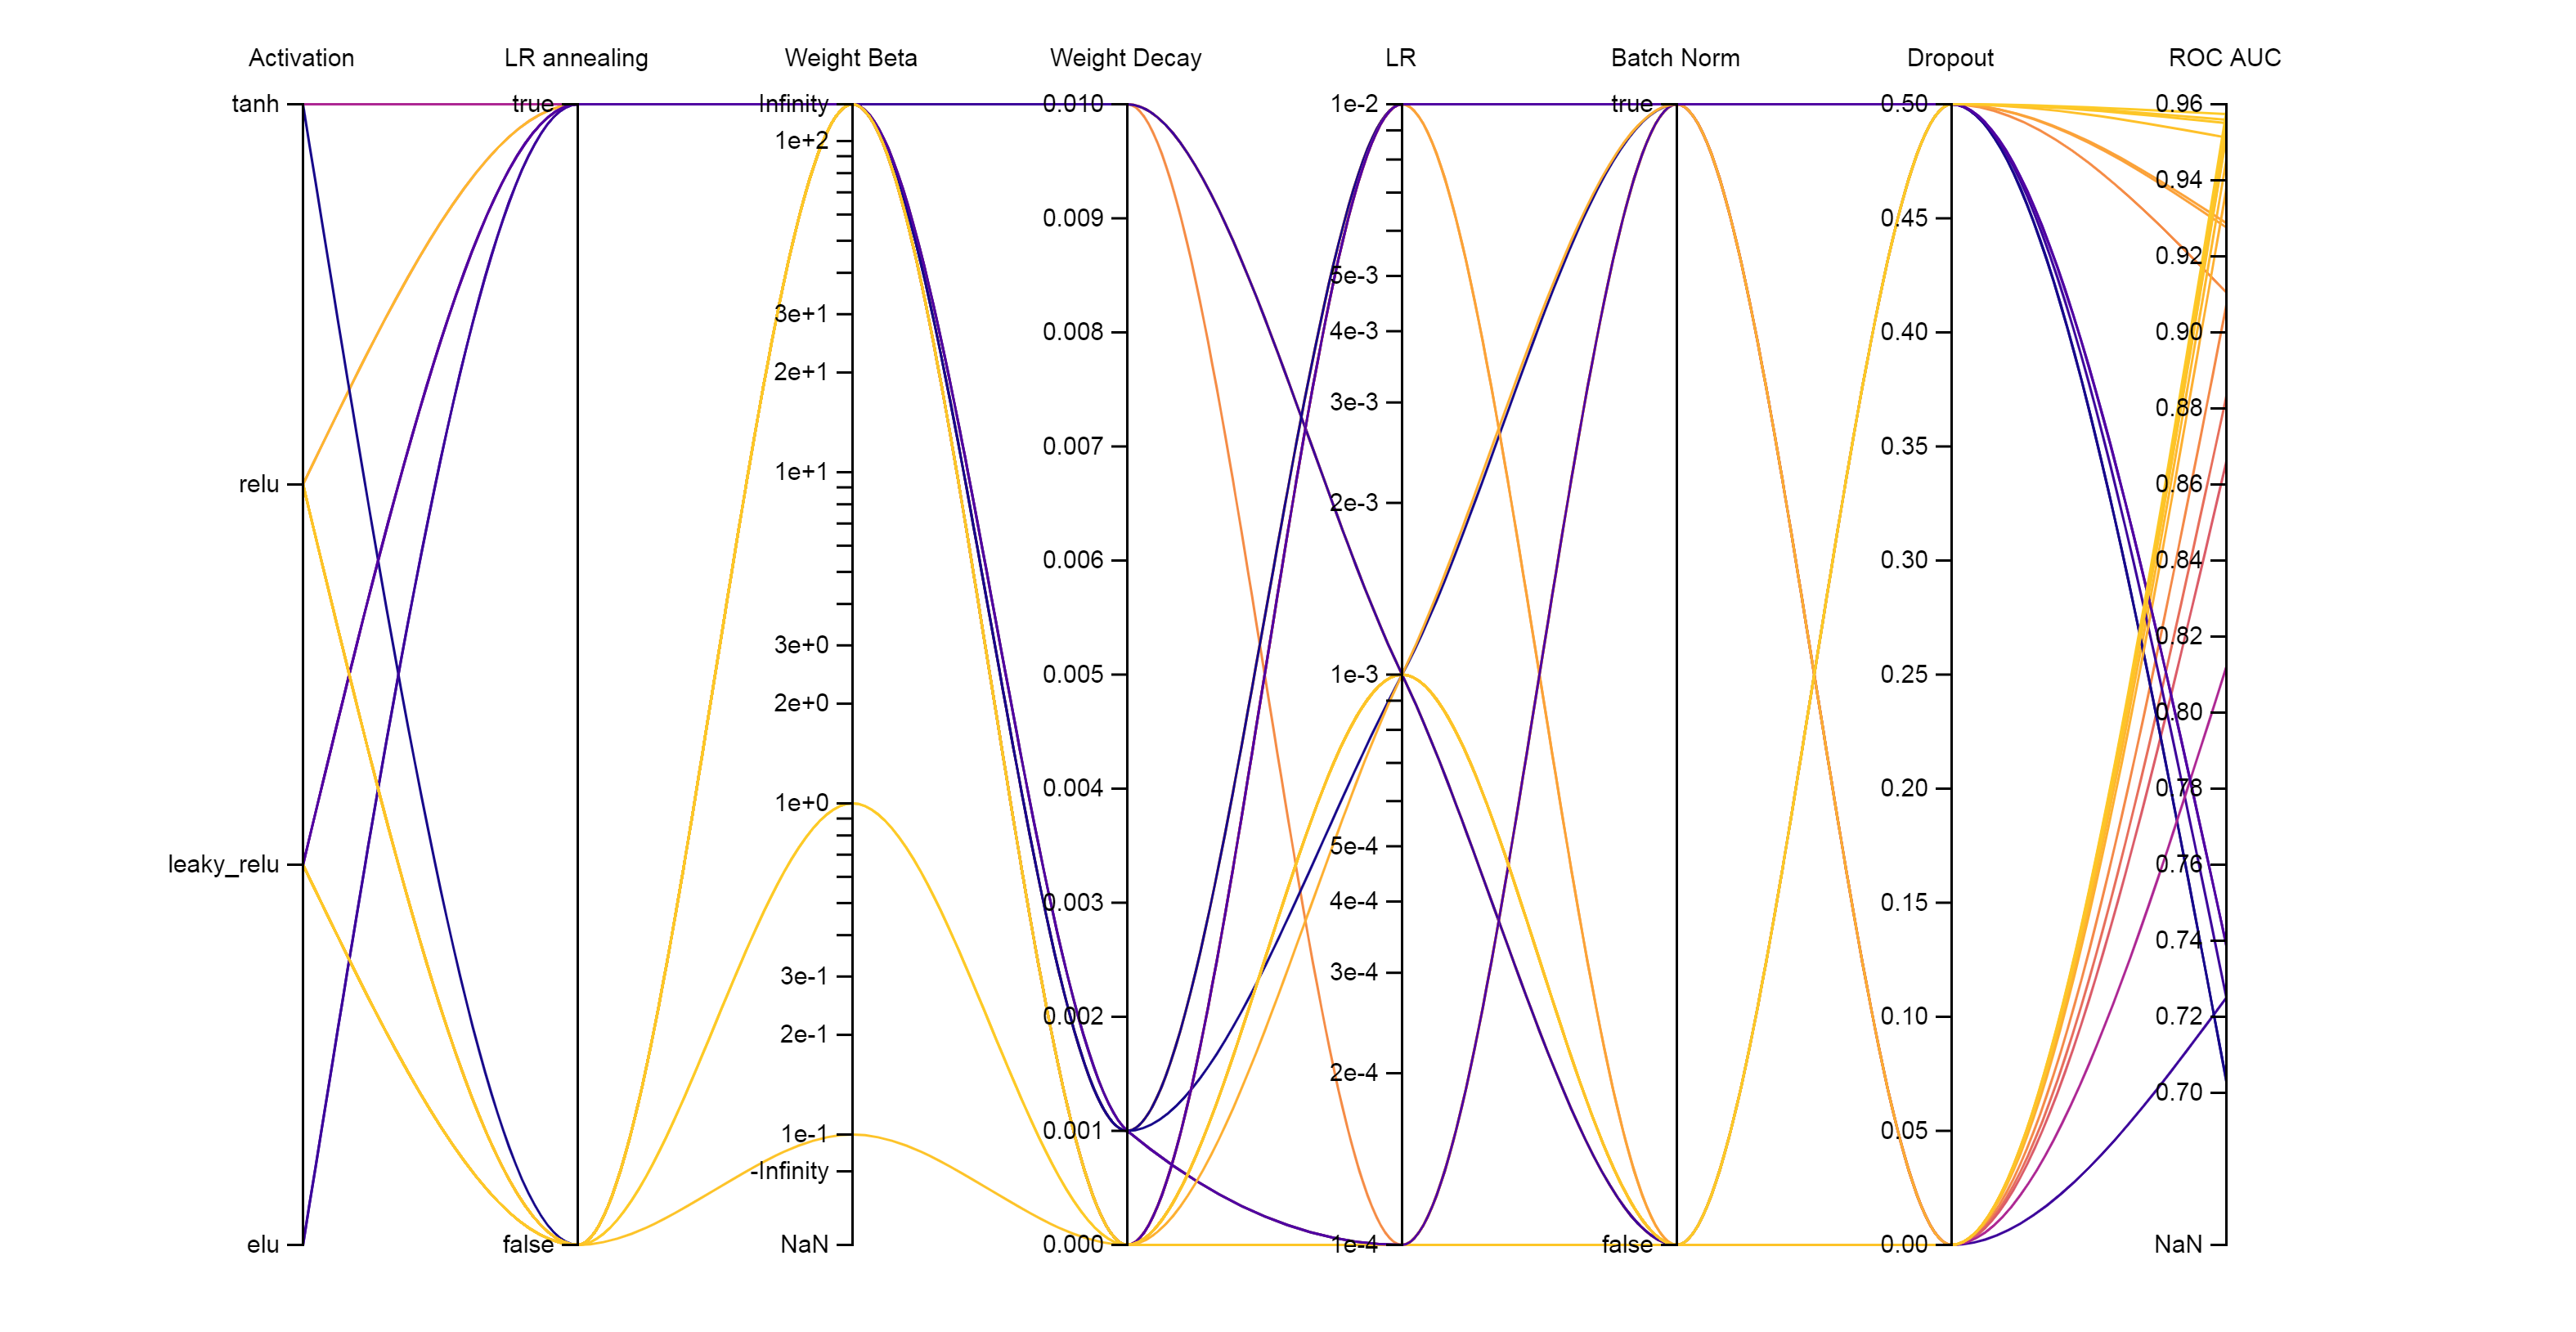
\includegraphics[width=\linewidth]{Section-0-Panel-0-5f4lnfvjk}}
\caption{Результаты экспериментов с различными гиперпараметрами}
\label{fig:run-waves}
\end{figure}

При переборе всех возможных наборов гиперпараметров валидационное качество не смогло значительно улучшиться. Однако, применение слоёв Batch Normalization и Dropout, а также взвешенных классов, помогают ускорить обучение модели без значительной потери валидационного AUC ROC. Как видно на \autoref{fig:batch-norm}, модели в среднем значительно раньше достигают своего пика, хотя и начинают намного раньше переобучаться, что характеризуется падением качества.
Также можно хорошо пронаблюдать эффект от добавления Dropout слоя на \autoref{fig:dropout}. Модель начинает медленее сходиться, но при этом модель не переобучается с резким падением качества. При добавлении этого слоя уменьшается разрыв между качеством на тренировочной и валидационной подвыборках.

\begin{figure}[h]
\noindent\makebox[\textwidth]{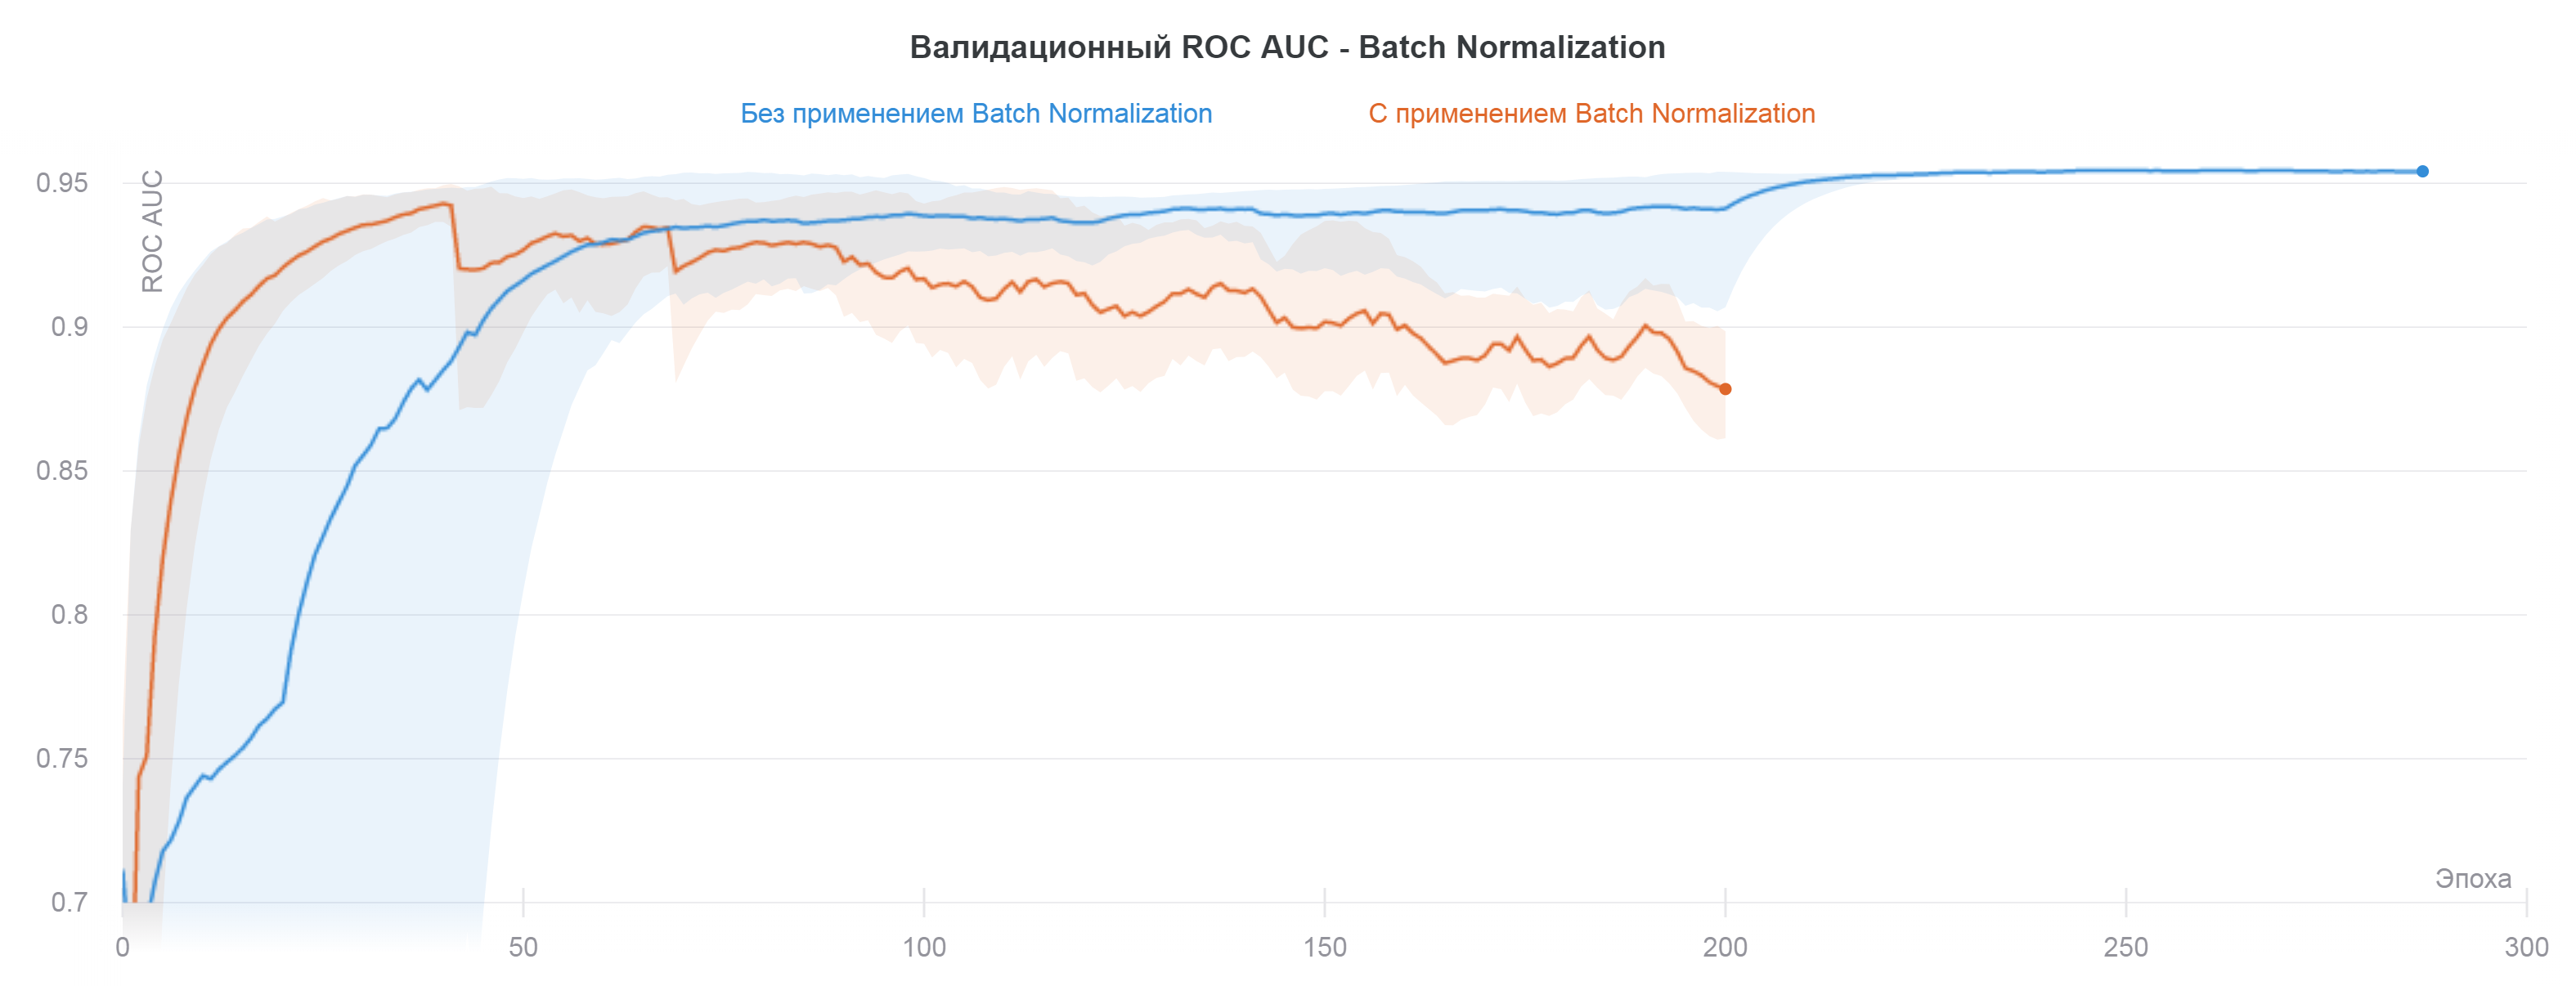
\includegraphics[width=\linewidth]{Section-0-Panel-2-wdsj85igb}}
\caption{Сравнение экспериментов с и без применения слоя Batch Normalization}
\label{fig:batch-norm}

\end{figure}
\begin{figure}[h]

\noindent\makebox[\textwidth]{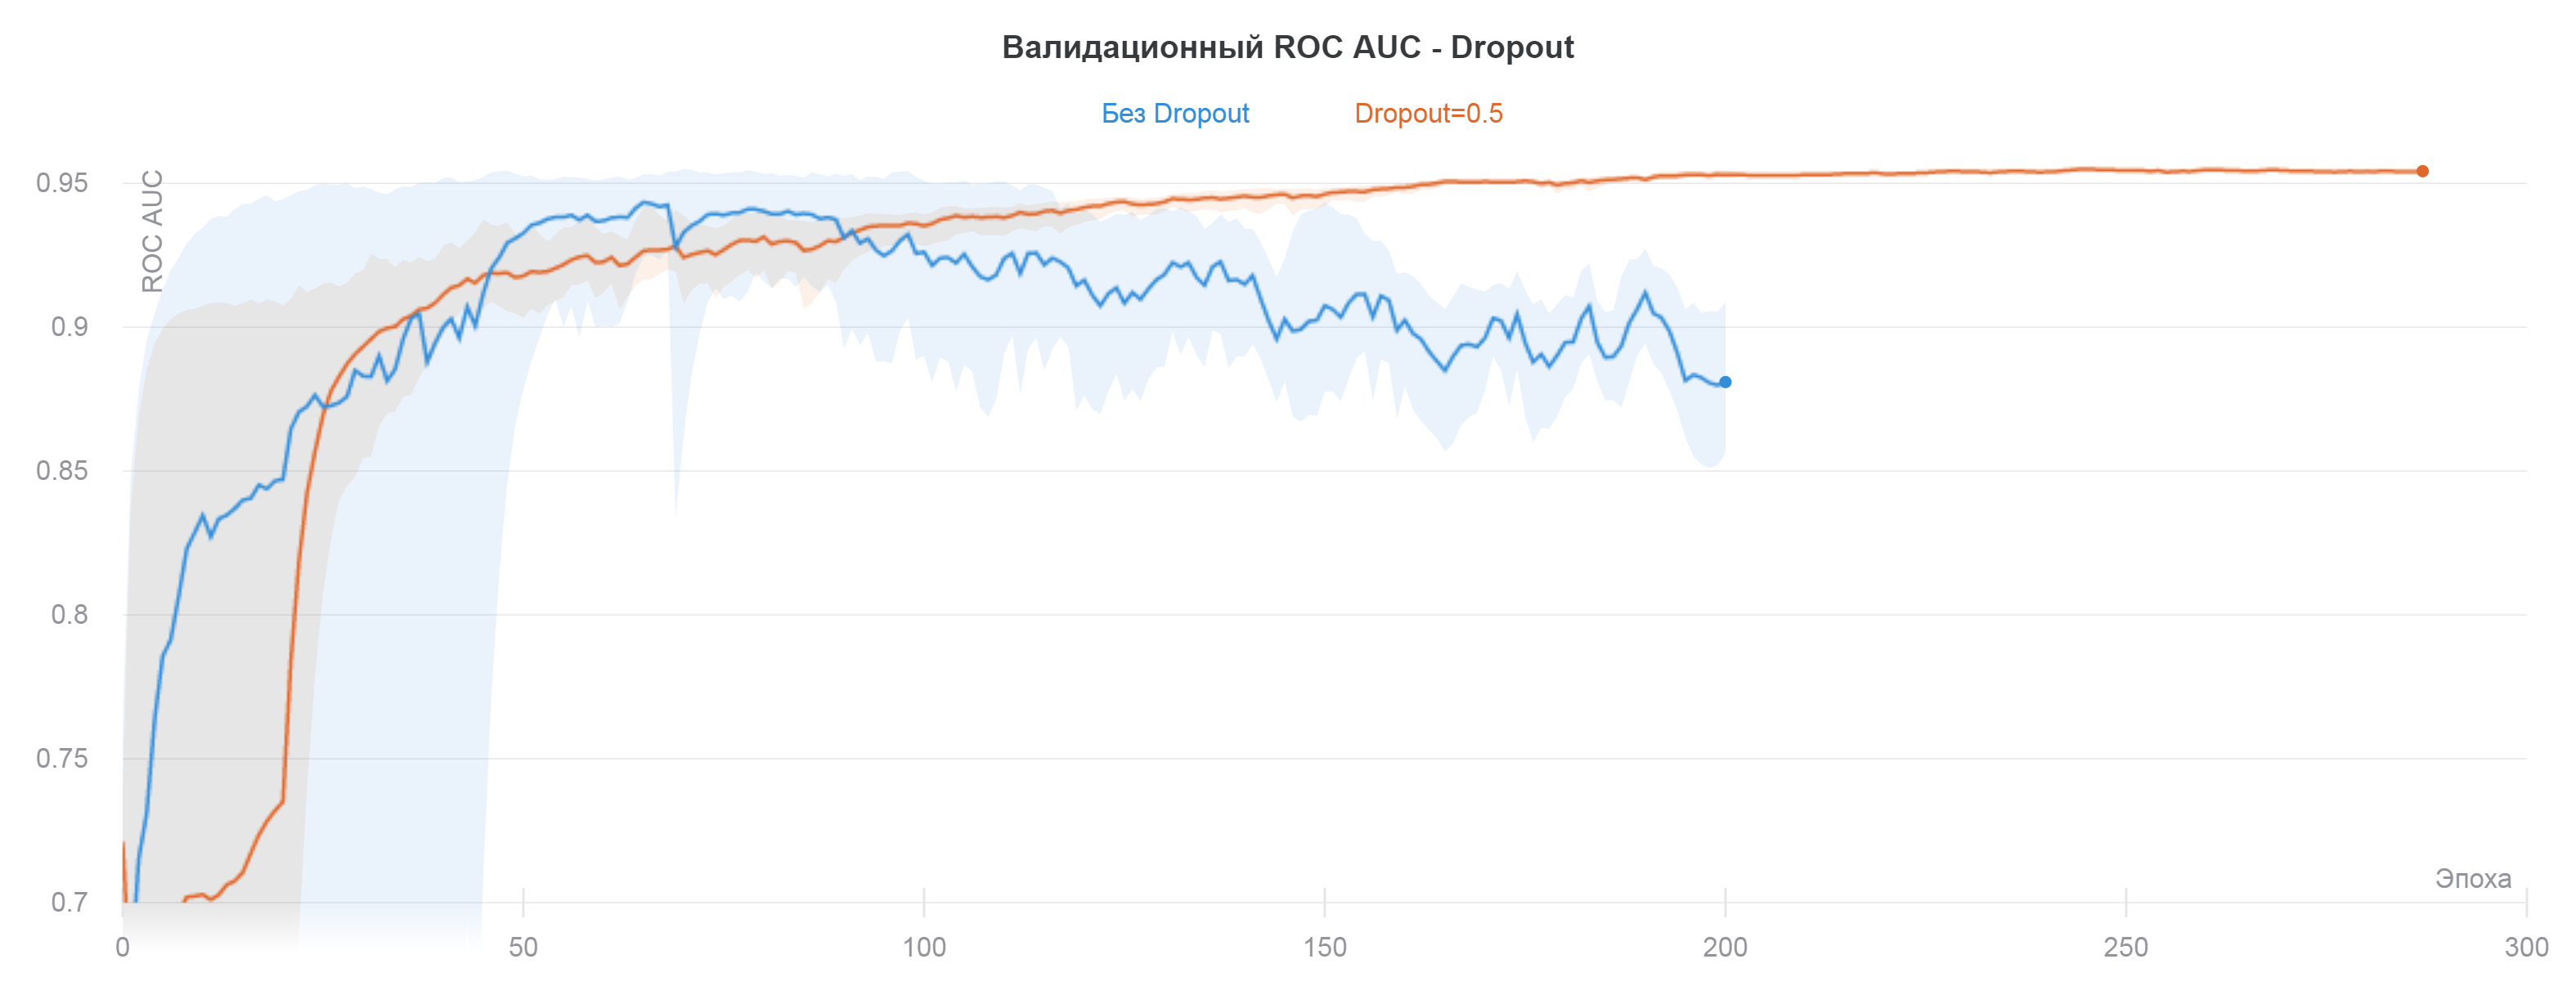
\includegraphics[width=\linewidth]{Section-0-Panel-3-ns9ivtwl4}}
\caption{Сравнение экспериментов с и без применения слоя Dropout}
\label{fig:dropout}

\end{figure}

При добавлении контентных данных, функция потерь у LSTM (\autoref{fig:lstm-loss}) и точность (\autoref{fig:lstm-accuracy}) на валидации несколько улучшаются. Однако, при использовании новых весов LSTM при обучении CNN, ROC AUC на валидации значительно падает.

\begin{figure}[H]

\noindent\makebox[\textwidth]{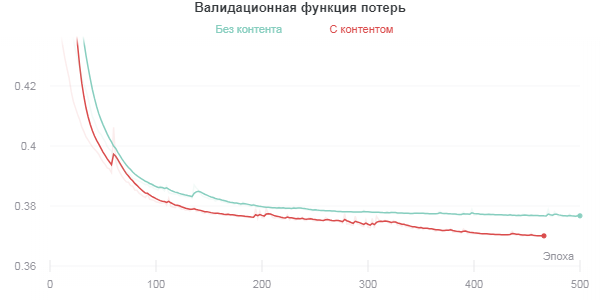
\includegraphics[width=\linewidth]{lstm-loss}}
\caption{Сравнение функции потерь при обучении LSTM с контентом и без}
\label{fig:lstm-loss}

\end{figure}
\begin{figure}[H]
\noindent\makebox[\textwidth]{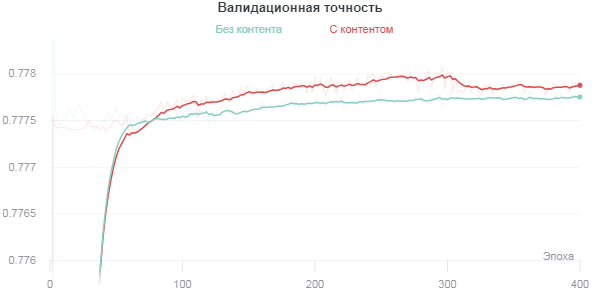
\includegraphics[width=\linewidth]{lstm-accuracy}}
\caption{Сравнение точности при обучении LSTM с контентом и без}
\label{fig:lstm-accuracy}

\end{figure}

Добавление Embedding-слоя в LSTM модель не оказало значимого влияния на качество предсказаний. Было попробовано два варианта обучения с этим слоем: обучение со случайной инициализацией вместе с обучением всей моделей, обучение весов слоя отдельно с помощью модели SkipGram. При обучении весов слоя с помощью SkipGram также есть два варианта: статический (веса Embedding-слоя фиксируются и не меняются при обучении LSTM) и динамический (веса Embedding-слоя дополнительно обучаются вместе с LSTM).\\
В итоге, ни один из вариантов Embedding слоя не улучшил результатов LSTM модели. Среди всех вариантов, статические SkipGram веса показали наилучший результат.


\chapter{Описание практической части}

\section{Выбранный инструментарий}

Для реализации использовался язык программирования Python версии 3.8, который был выбран в силу своего удобство и простоты. Также важным преимуществом этого языка является наличие множества дополнительных программных модулей с открытым программным кодом.\\
Проект включает в себя Python-скрипты, а также Jupyter блокноты. Jupyter - среда для интерактивного программирование, которое упрощает осуществление экспериментов.\\
В качестве ключевых фреймворков и программных модулей, используемых для реализации проекта, можно выделить:
\begin{itemize}
\item PyTorch \cite{NEURIPS2019_9015} - популярный фреймворк для создания и обучения нейросетей, разрабатываемые компанией Facebook. Ему было отдано предпочтение, потому что, в отличие от его единственного конкурента TensorFlow, PyTorch обладает качественными документацией и программным интерфейсом, что делает разработку и поддержание моделей более простым и удобным;
\item Scikit-learn \cite{scikit-learn} - программный модуль, содержащий в себе огромное количество различных классических алгоритмов машинного обучения и различные средства обработки данных. Был взят именно он, потому что является де-факто стандартом в своей сфере;
\item Pandas \cite{mckinney-proc-scipy-2010} - модуль для работы со табличными массивами данных. Используется, так как предлагает множество инструментов, облегчающие работу с csv-файлами из набора данных;
\item Dask \cite{dask} - модуль для параллелизированной обработки данных. Имеет программный интерфейс схожий с Pandas. Предназначен для агрегации данных с контентом, размеры которых превышают доступную оперативную память на рабочей машине;
\item Ignite - надстройка для PyTorch, упрощающая написание процесса обучения и валидации моделей;
\item GenSim \cite{rehurek_lrec} - модуль для работы с текстовыми данными. Взят, так как он способен работать с огромными массивами текстовых данных, которые не способны уместиться в оперативной памяти;
\item TensorBoard - модуль для логирования обучения моделей. Так как является частью проекта TensorFlow, используется модуль TensorBoardX, который предоставляет программный интерфейс для любых фреймворков;
\item Weights and Biases \cite{wandb} - сервис для сбора логов и результатов экспериментов и их последующей визуализации. Для этого предоставляется Python модуль wandb.
\end{itemize}

За неимением адекватной видеокарты, для обучения нейросетей используется сервис Google Colaboratory, который предоставляет бесплатный доступ к онлайн Jupyter-ноутбукам в средах с доступом к производительным GPU. Сервис обладает рядом ограничений на время работы и зачастую сервис нестабилен, но для обучения рассматриваемых моделей этого достаточно.

\section{Сценарии функционирования}

Проект включает в себя один базовый сценарий построения моделей машинного обучения для классификации пользовательского поведения и проведения экспериментальных исследований. Этот сценарий разбивается на несколько:
\begin{itemize}
	\item Составление признакового описания данных;
	\item Обучение SkipGram-модели;
	\item Обучение LSTM-кодировщика;
	\item Обучение CNN-классификатора.
\end{itemize}

% TODO Написать про SkipGram в обзоре

Для обучения любых моделей требуются подготовленные признаковые описания данных. На этом же этапе происходит разделение данные на тренировочные и валидационные подвыборки. Обучение SkipGram моделей используется как опциональный компонент, в то время как для обучения CNN-классификатора, требуется уже обученная LSTM-модель. Обучение всех моделей происходит по эпохам. В конце каждой тренировочной эпохи вычисляются метрики по тренировочной и валидационной подвыборках. Все полученные метрики собираются в лог-файл. Также в конце каждой эпохи происходит сохранение полученных весов моделей, если модель является лучшей по валидационной метрике. Обучение продолжается до тех пор, пока количество эпох не превысит вручную заданный порог, или в случае, если в последние N эпох валидационные метрики не улучшались (техника, которая называется ``ранней остановкой'').

\section{Архитектура разработанного средства}

Разработанный проект делится на подготовленные программные модули, в которых описываются тестируемые модели, конфигурации, схема обработки данных, процесс обучения моделей. Также есть Jupyter-тетради, в которых происходят эксперименты с моделями в интерактивном режиме.\\
На \autoref{fig:architecture} условно отображена архитектура программного средства. В круглых облаках написаны названия классов, направленные стрелки обозначают наследование классов, а не направленные - ассоциацию классов. В пунктирных коробках отображаются Jupyter-тетради, в которых проводятся эксперименты и используемые методы из других модулей.

% TODO: update line count
Всего написано \textbf{2443} строк кода, которые включают в себя \textbf{1034} строк в python-скриптах и суммарно \textbf{1409} строк кода в ячейках Jupyter-тетрадей.\\

\begin{figure}[ht]
	\noindent\makebox[\textwidth]{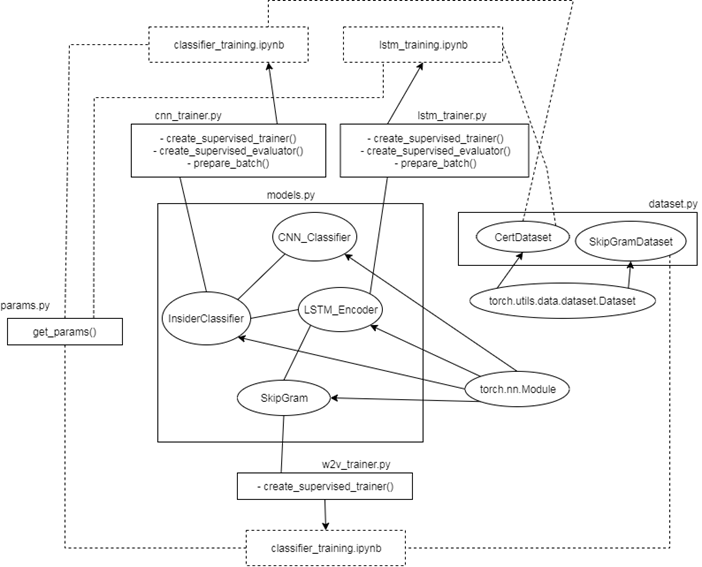
\includegraphics[width=\linewidth]{architecture-scheme}}
	\caption{Архитектура разработанного средства}
	\label{fig:architecture}
\end{figure}

Разработанные программные модули:
\begin{itemize}
\item Для каждого типа обучаемых нейросетей, есть \textit{``xxx\_trainer.py''} скрипт, который описывает процессы обучения и валидации модели. С помощью средств модуля Ignite устанавливаются функции обратного вызова и события, при которых они вызываются. С помощью этих функций происходит вычисление вспомогательных метрик, TensorBoard логирование, сохранение на жёсткий диск промежуточных, финальных и лучших по валидации весов модели. Скрипты обладают функциями \textit{create\_supervised\_trainer()} описывающие процесс тренировки; \textit{create\_supervised\_evaluator()}, которая описывает процесс валидации и \textit{prepare\_batch()}, описывающее процесс обработки полученных данных для текущей задачи. Каждому скрипту соответствует файл Jupyter-тетради \textit{``xxx\_training.ipynb''} в которых проводятся эксперименты с соответствующей моделью.
\item{``\textit{dataset.py}''} описывает обработку данных. Реализовано два класса: \textit{CertDataset} и \textit{SkipGramDataset} для обучения классификатора и SkipGram модели соответственно. Оба класса наследуются от класса \textit{utils.data.dataset.Dataset} из фреймворка Pytorch.
\item ``\textit{models.py}'', который описывает архитектуру обучаемых моделей. Каждая модель задаётся специальным Python-классом, унаследованным от класса из пакета Pytorch nn.Module. В каждом классе описываются методы \textit{\_init\_()} (конструктор, в котором описываются поля объекта и задаются слои модели) и \textit{forward()}, в которой происходит обработка объектов, поступивших на вход модели. Реализованные классы: \textit{CNN\_Classifier}, \textit{LSTM\_Encoder}, \textit{InsiderClassifier} и \textit{SkipGram}, которые описывают CNN-классификатор, LSTM-кодировщик, классификатор инсайдерского поведения целиком и SkipGram-модель соответственно. \textit{InsiderClassifier} содержит в себе модели \textit{CNN\_Classifier} и \textit{LSTM\_Encoder}.
\item ``\textit{params.py}'' - содержит в себе конфигурацию для обучения моделей и подготовки данных. Реализован в виде простого Python-скрипта, который содержит в себе многоуровневый ассоциативный массив с параметрами. Обладает только функцией \textit{get\_params()}, которая выводит параметры эксперимента.
\end{itemize}


\chapter{Заключение}

В данной работе было изучено множество актуальных средств решения проблемы автоматического обнаружения инсайдерских угроз на основе анализа поведенческих данных. Также были рассмотрены различные наборы данные, содержащие в себе информацию о пользовательском поведении.\\

В результате обзора набора данных был взят набор CMU CERT версии 4.2. В качестве валидационнной метрики был выбран ROC AUC. По итогу обзора существующих решений, для последующей работы была выбрана модель состоящая из LSTM-кодировщика и CNN-классификатора.
\\
Для сравнения также был использован ряд классических классификаторов (логистическая регрессия, SVM, KMeans, случайный лес). Модель со сверточным классификатором показала наилучшую метрику AUC ROC \textbf{0.9566}.\\

Был предложен ряд улучшений для существующего решения, которое позволяет достичь большей валидационной метрики. Как показали эксперименты, для обучения CNN-классификатора очень критична проблема переобучения. Использование слоёв batch-нормализации, взвешенной функции потерь и Dropout-слоев позволяют с этим бороться, значительно ускоряя сходимость нейросети и улучшая качество предсказаний. Лушчее качество AUC ROC из всех экспериментов - \textbf{0.9574}\\

Добавление тем контента не улучшило качество классификации до AUC ROC \textbf{0.9021}. Это возможно в силу синтетической природы набора данных или недостаточной обобщающей способности классификатора.

\nocite{*}
\bibliographystyle{gost780u}
\bibliography{0-main}


% \listoftodos[Notes]

\backmatter %% Здесь заканчивается нумерованная часть документа и начинаются ссылки и
            %% заключение

\appendix   % Тут идут приложения

\end{document}
